\chapter{Networks}

\newthought{Networks are structures describing connections between elements.} For example, Twitter followers are a network describing who follows whom. Proteins interact with one another, which can be shown in a network, where protein interactions are connections between elements. Citations in text are a network, in which authors reference one another. And so on.

Elements in a network are called nodes. You can imagine nodes as rows in the data (i.e. Twitter users, proteins, authors). Connections between these elements are called edges (i.e. following someone, protein interaction, citation).

\section{Installing the Network add-on}

You will need the \emph{Network add-on}, which introduces components for network visualization and analysis. To install Network add-on, go to Options --> Add-ons and select Network from the list. You will have to restart \mutation for widgets to appear.

A new pane with widgets from the Network add-on will appear on the left side of the canvas.

\section{Loading networks}

Let us observe a simple network. With the \widget{Network File} widget, go to \emph{Browse documentation networks...} and select \emph{lastfm.net} from the list. Lastfm\marginnote{Lastfm network is derived from the Lastfm website, where users can tag tracks with labels. Here, \emph{best tag} corresponds to the most frequent tag for the artists, and edges are the number of shared tags.} describes a network of artists and the genre they most likely belong to. Nodes in the network are artists, while edges are shared tags.

\vspace{-0.2cm}
\begin{figure}[h]
  \centering
  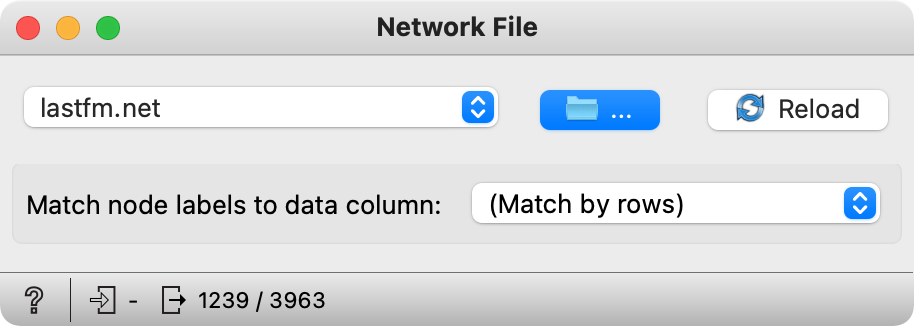
\includegraphics[width=\linewidth]{network-file.png}%
  \caption{$\;$}
\end{figure}
\vspace{-0.3cm}

\newpage

\section{Visualizing networks}

One can, of course, observe the data in a \widget{Data Table}, but in case of networks, all one would see are metadata. A better way of exploring networks is with \widget{Network Explorer}. This visualization shows network structure with points being artists, colored by the most frequent genre tag.

\vspace{-0.2cm}
\begin{figure}[h]
  \centering
  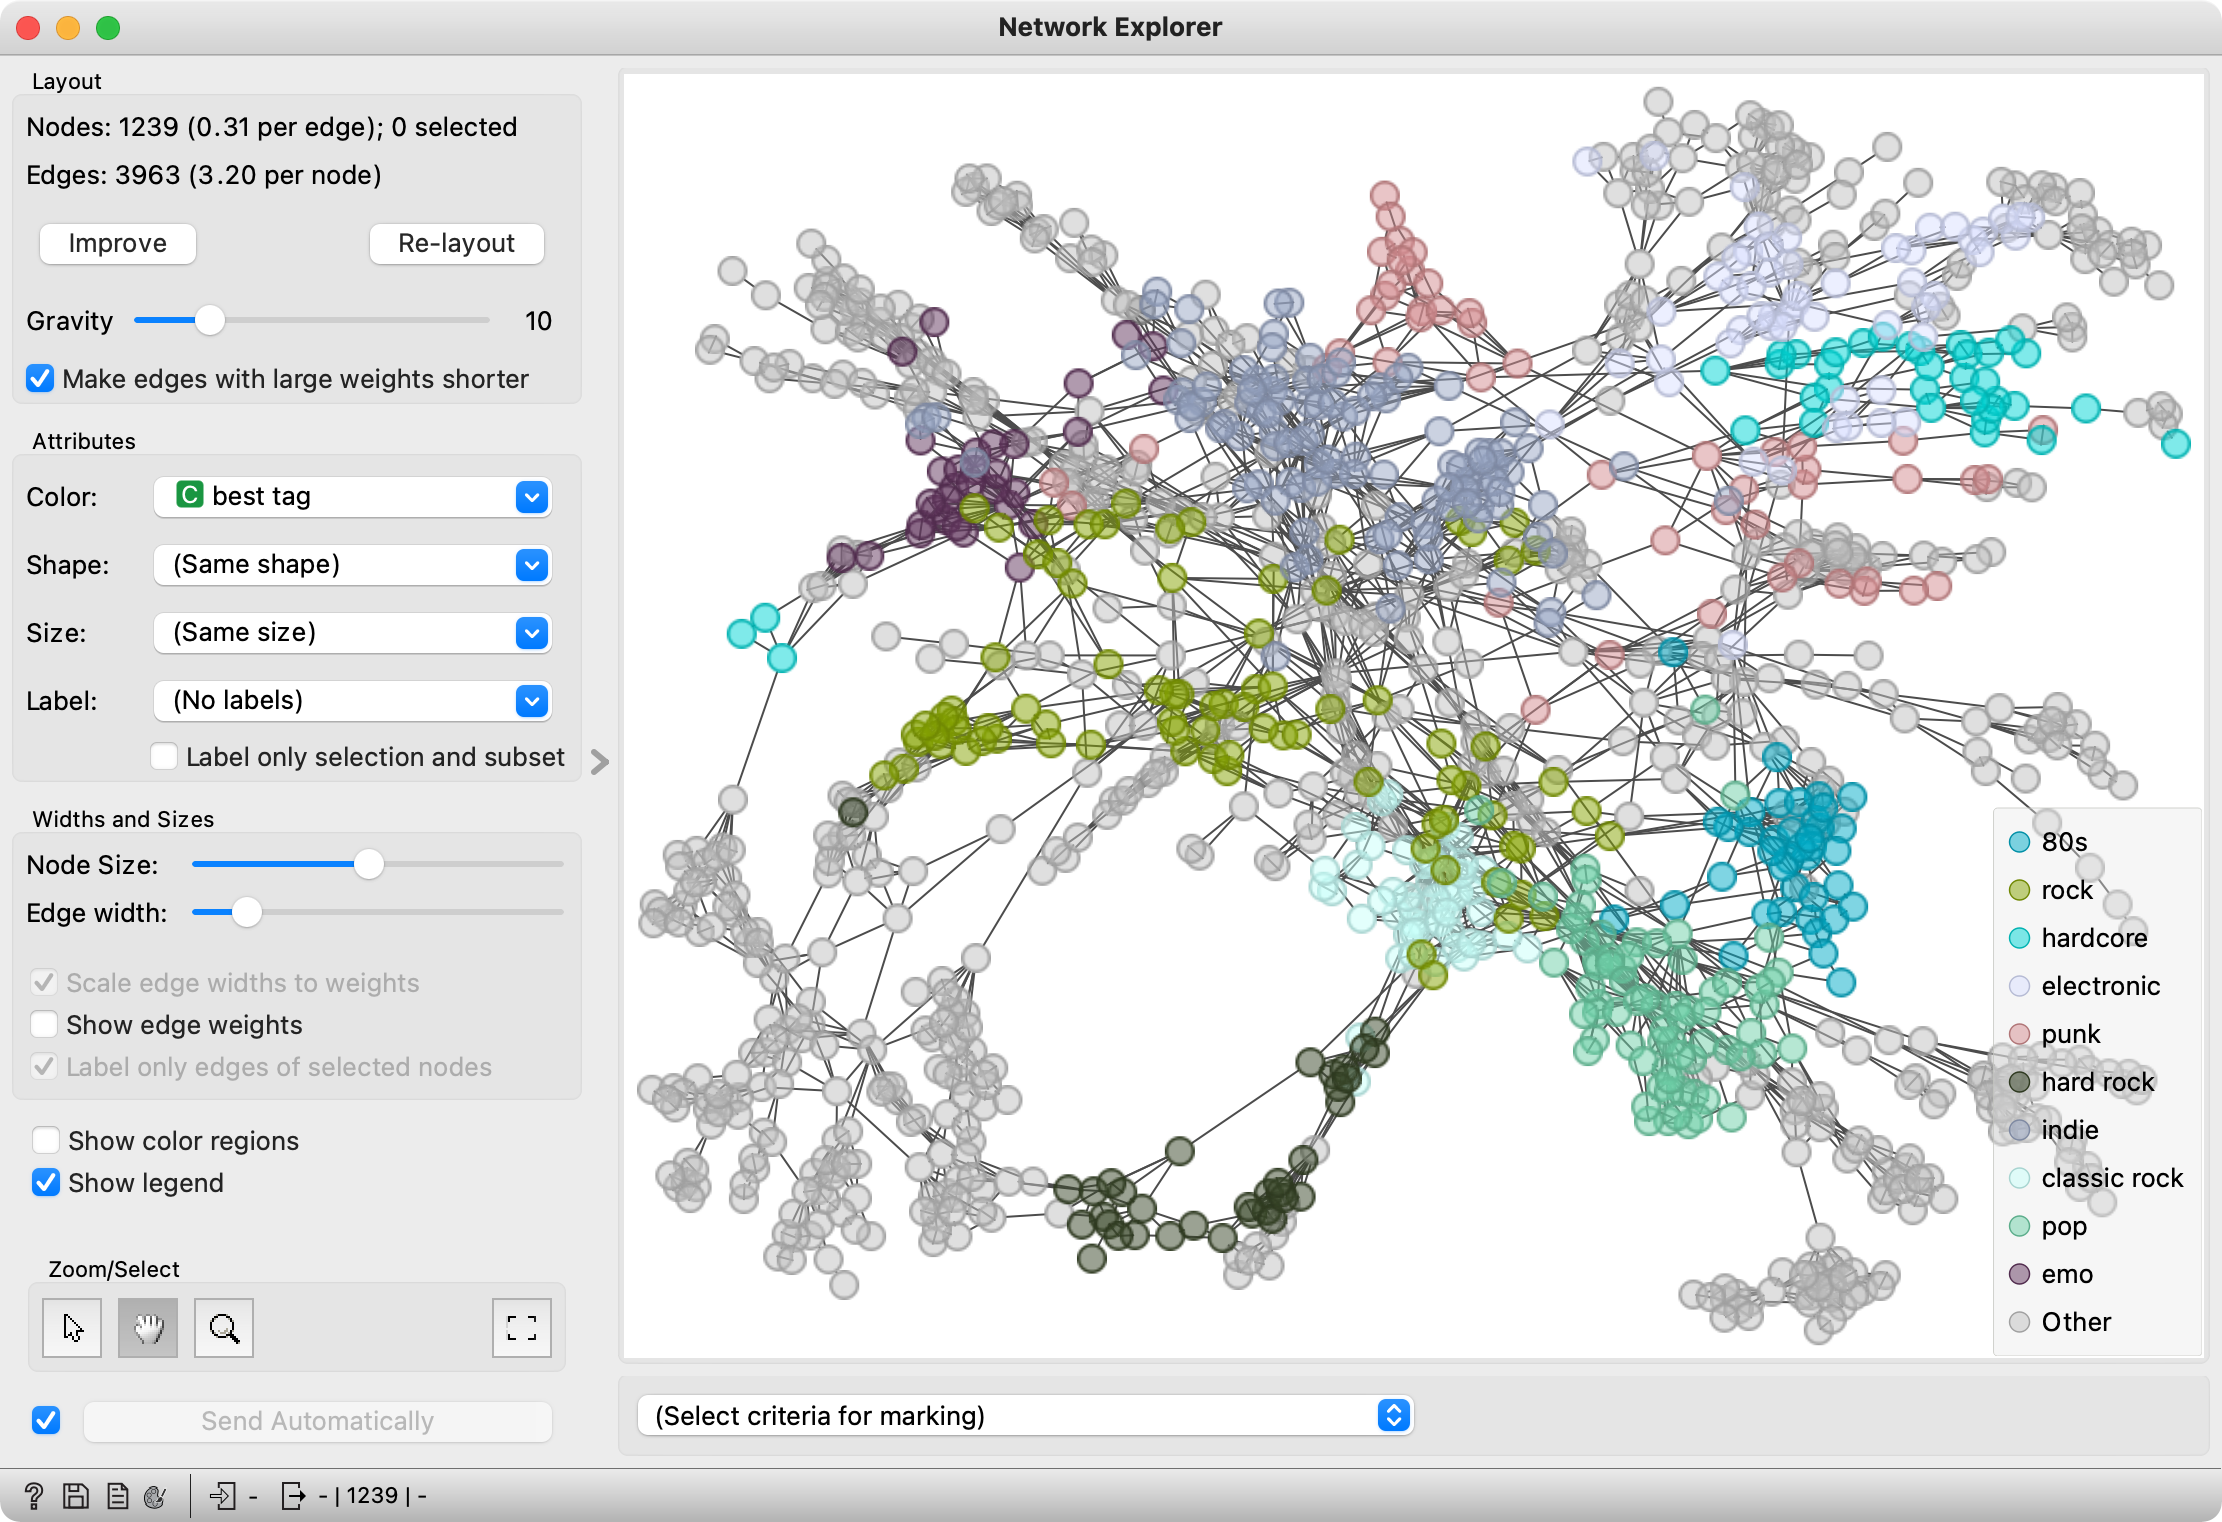
\includegraphics[width=\linewidth]{network.png}%
  \caption{$\;$}
\end{figure}
\vspace{-0.3cm}

% \begin{marginfigure}
%       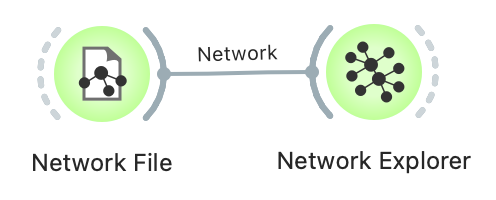
\includegraphics[width=30mm]{workflow.png}%
%       \caption{$\;$}
% \end{marginfigure}

Now let us zoom in onto a genre, say the 80s. We will turn on the \emph{Show color regions} options, which will color the plot by the prevalent tag. Seems like the 80s are in close connection to pop artists.

\vspace{-0.2cm}
\begin{figure}[h]
  \centering
  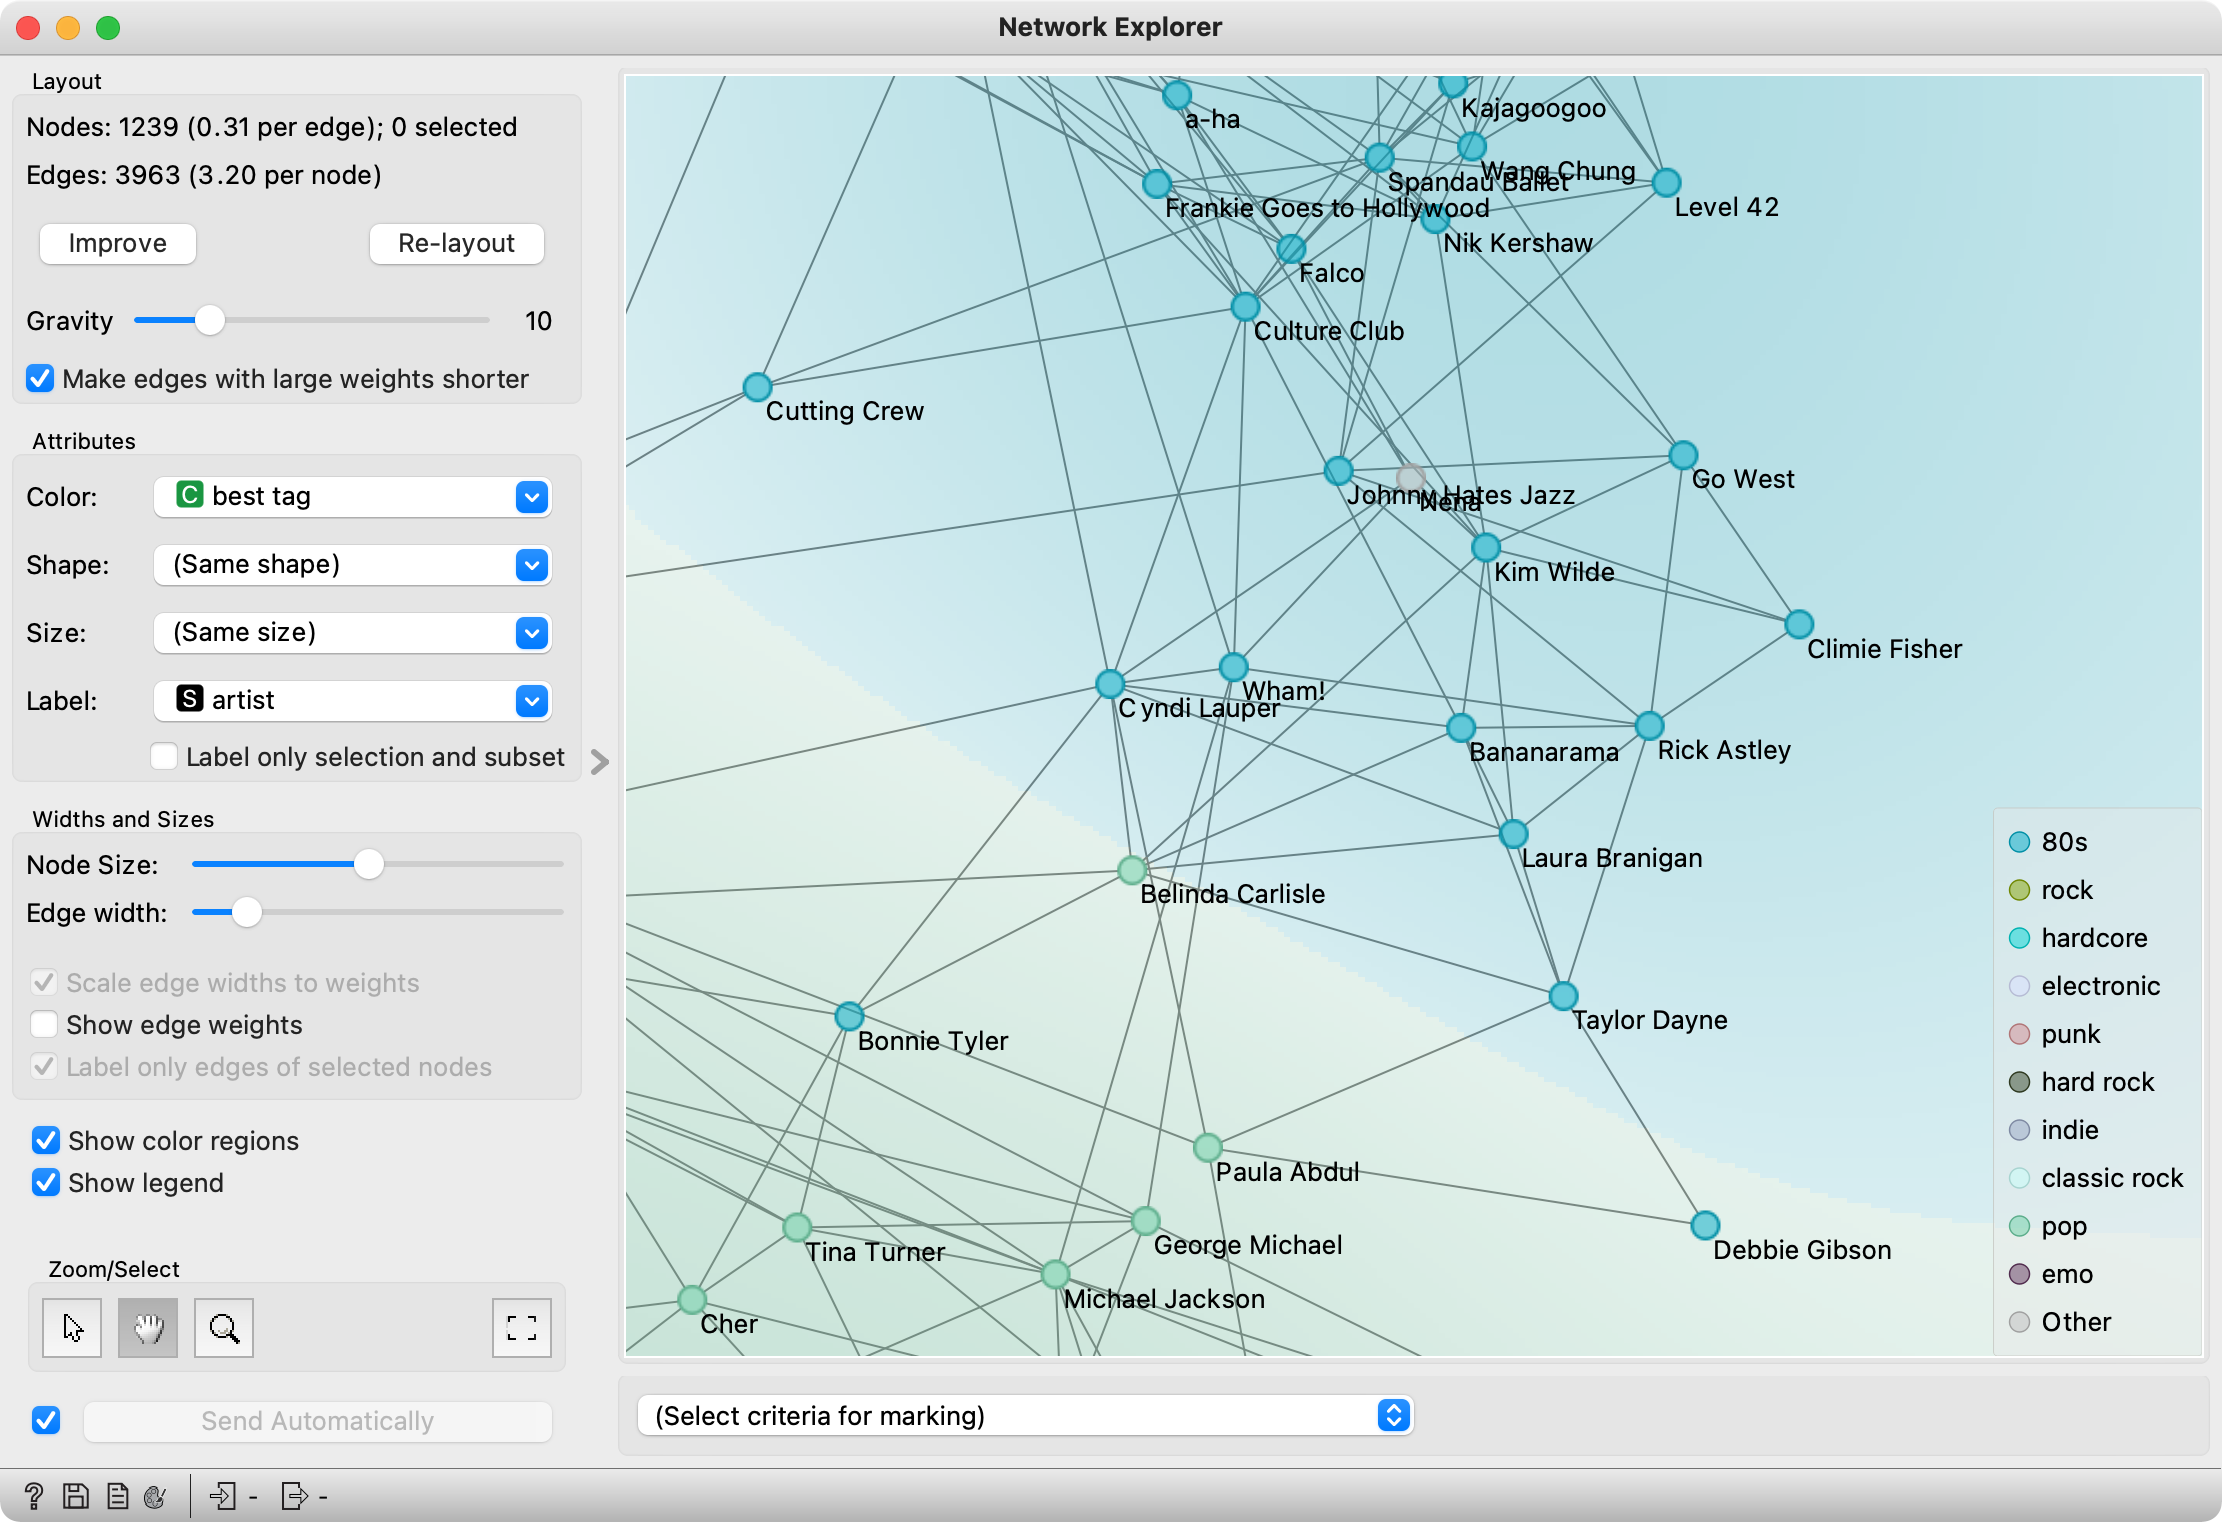
\includegraphics[width=\linewidth]{network-zoom.png}%
  \caption{$\;$}
\end{figure}
\vspace{-0.3cm}

\newpage

But who are the genre representatives? If a node shares many similar tags with its neighbors, this would likely be the most typical representative of the genre. Let us select those nodes from the graph. At the bottom of the widget, set selection criteria to \emph{Mark nodes with more connections that any neighbor}, then press \emph{Select} to send the selection to the output.

\vspace{-0.2cm}
\begin{figure}[h]
  \centering
  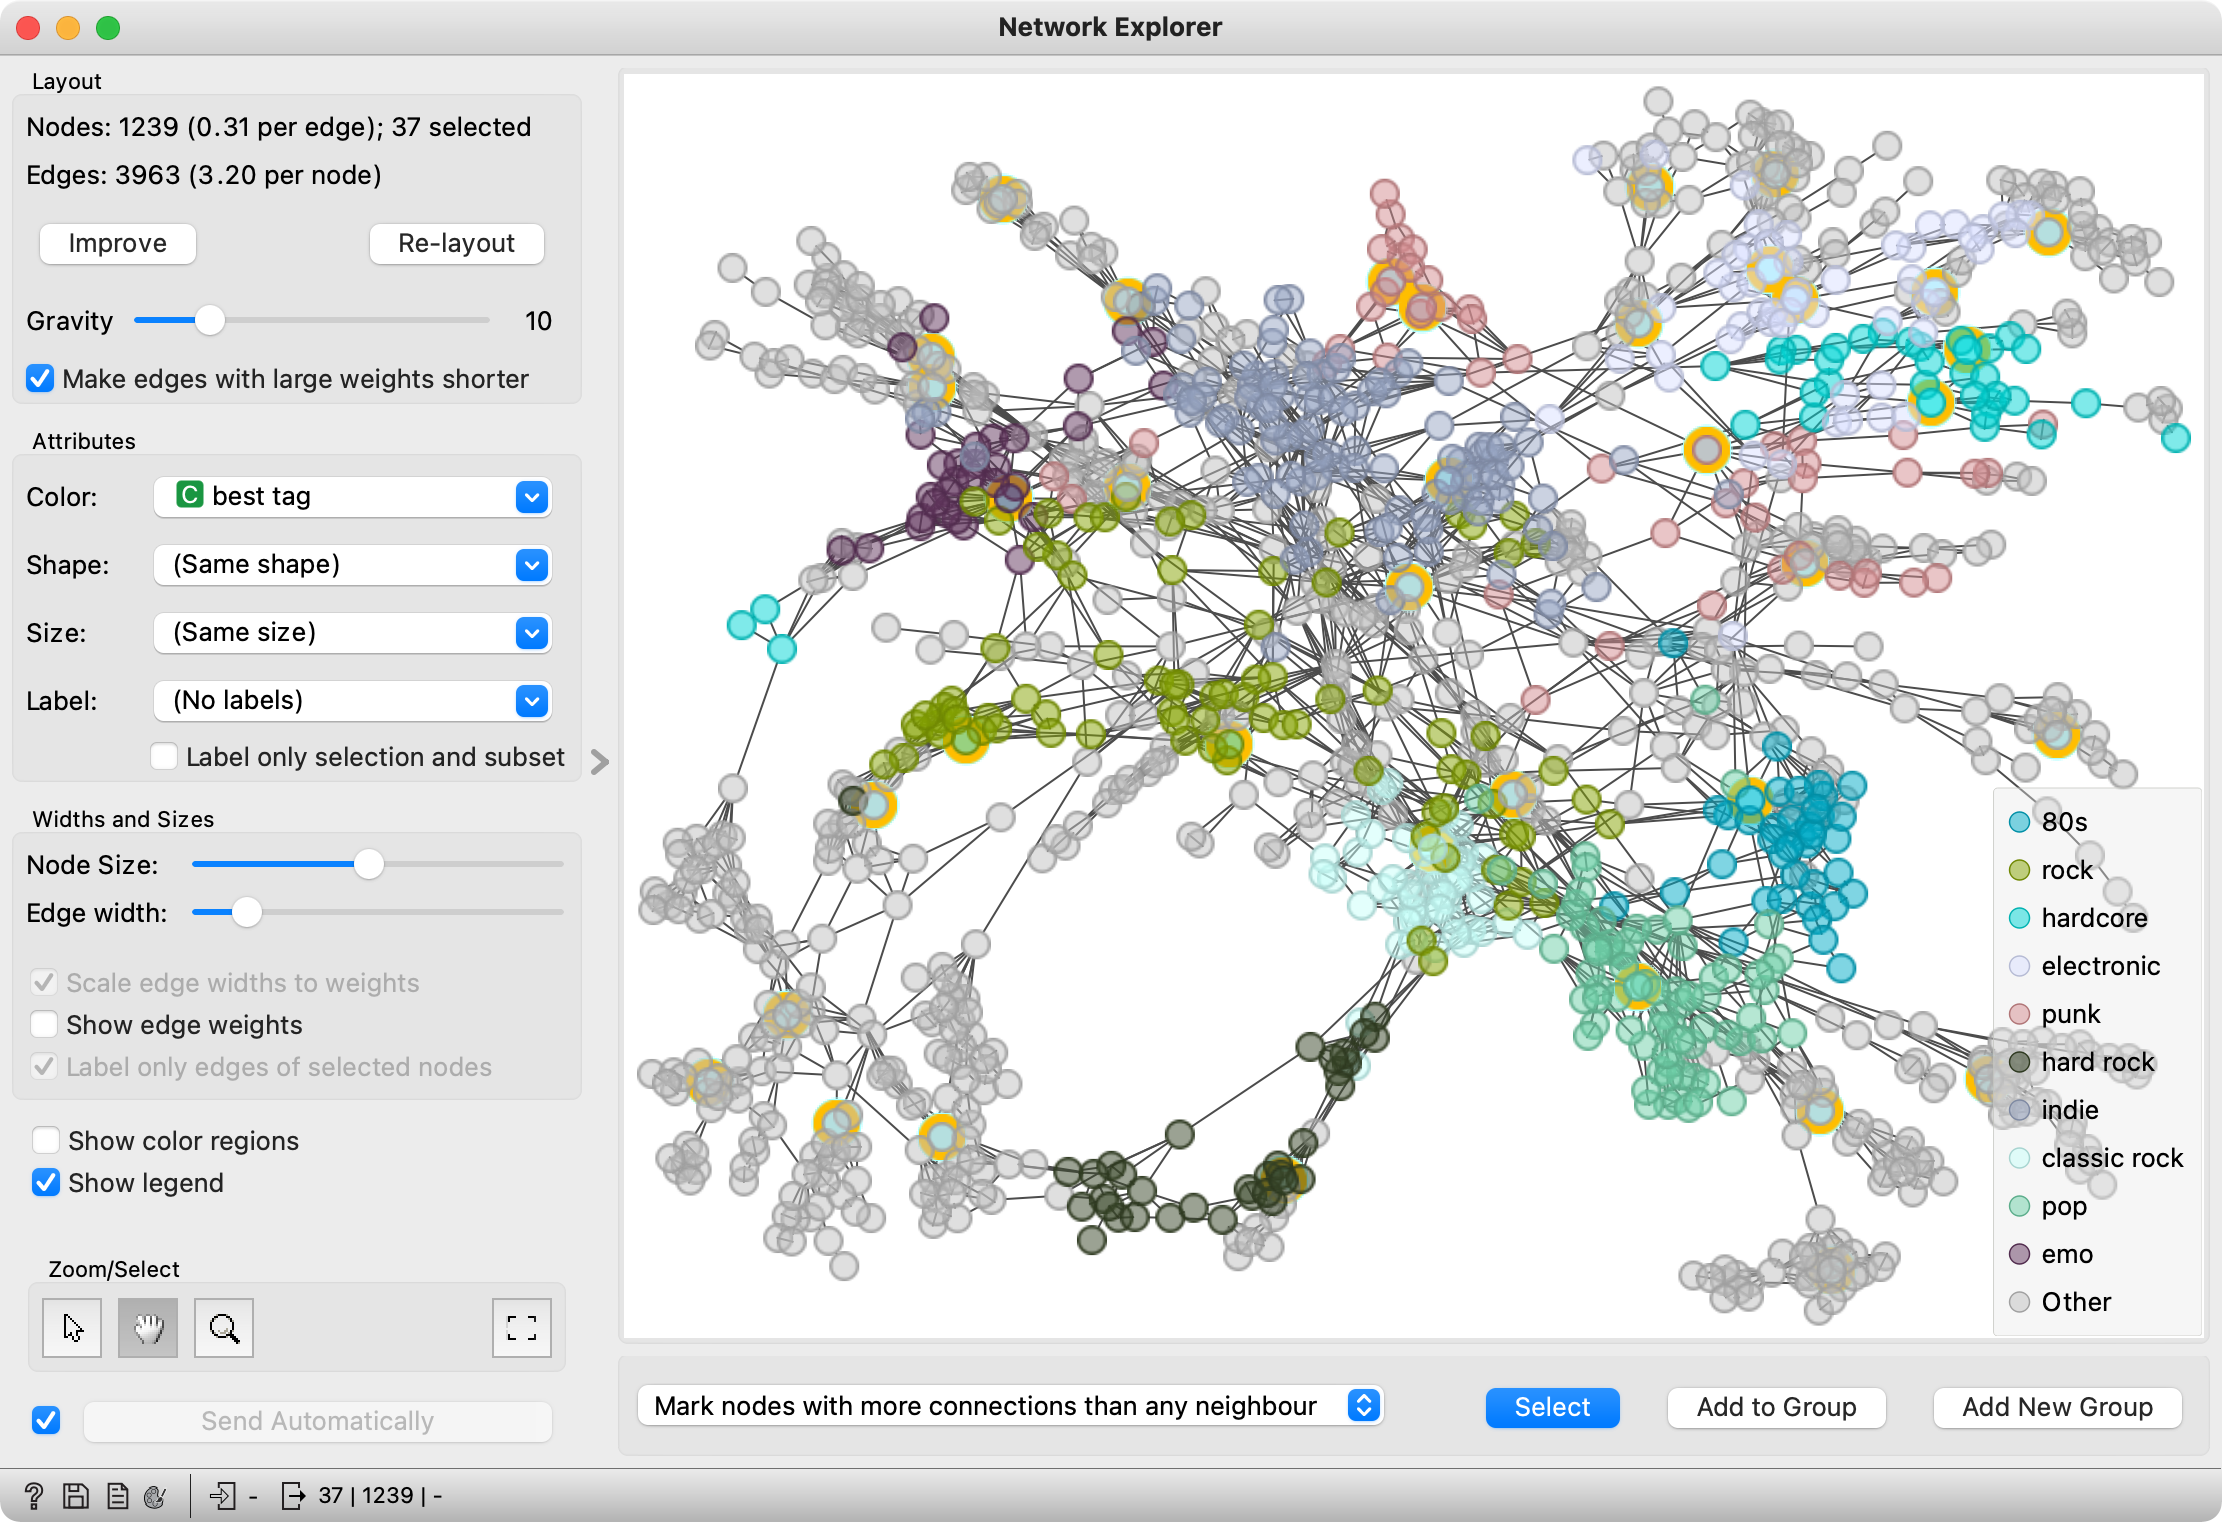
\includegraphics[width=\linewidth]{network-selection.png}%
  \caption{$\;$}
\end{figure}
\vspace{-0.3cm}

Connect \widget{Data Table} to the widget and observe the subset. The Rolling Stones as typical classic rock representatives and Britney Spears as a typical pop artist? Sounds about right.

\vspace{-0.2cm}
\begin{figure}[h]
  \centering
  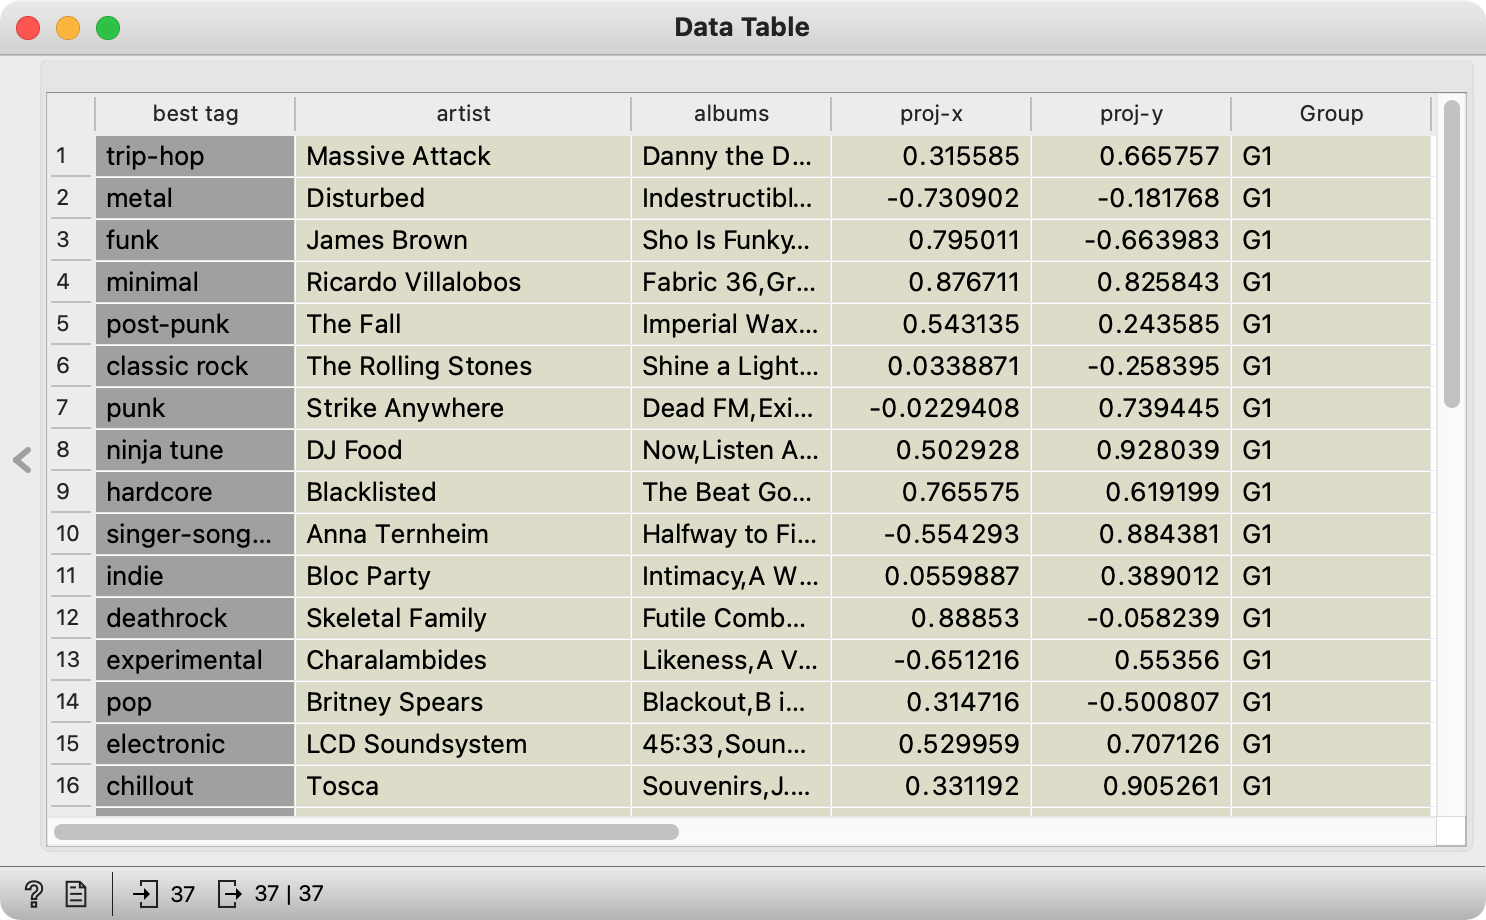
\includegraphics[width=\linewidth]{data-table.png}%
  \caption{$\;$}
\end{figure}
\vspace{-0.3cm}
